\chapter{Estado de la Cuestión}
\label{cap:estadoDeLaCuestion}
En este capítulo se hará una investigación sobre las técnicas, herramientas y formas de crear inteligencias artificiales para enemigos.
Para ello vamos a comenzar haciendo un recorrido por todo lo relacionado con la inteligencia artificial en general y cómo se usa esta en videojuegos 2D de plataformas, ya sea para crear un NPC, un enemigo o para optimizar alguna función más a bajo nivel del juego.
Se mencionarán además herramientas para conseguir los fines descritos anteriormente y se hablará de algunos motores de videojuegos que han inspirado en cierta manera algunos aspectos de nuetras herramienta. \\
\section{Introducción a la Inteligencia Artificial}

La Inteligencia Artificial (IA) es la capacidad que tiene un sistema o software de realizar tareas diferentes entre sí de manera autónoma aplicando reglas, algoritmos o patrones de aprendizaje automático, simulando así comportamientos propios de la inteligencia humana.
El potencial de la IA hoy día y por lo que está generando tanto furor es su capacidad de autonomía, ya que no solo sigue reglas, si no que tiene la capacidad de tomar decisiones\\
En el ámbito de los videojuegos, la IA se ha hecho paso a base de demostrar su gran capacidad de adaptación a contextos diversos como la adaptación del Alien en \textit{Alien Isolation}\footnote{\url{https://www.gamedeveloper.com/design/the-perfect-organism-the-ai-of-alien-isolation}} , la manera en la que puede generar contenido procedural para juegos roguelike como \textit{Hades}\footnote{\url{https://hades.fandom.com/es/wiki/Hades_(juego)}} o ,por último, entrenar una IA para que se acerque lo máximo posible al comportamiento de un humano como en la serie \textit{Forza Motosport}\footnote{\url{https://forza.fandom.com/wiki/Forza_Wiki}}, usando redes neuronales.\\
\section{Tecnicas}

Es muy importante a la hora de escoger una técnica para modelar la IA de una entidad el saber ciertos factores para tomar la decisión correcta, como por ejemplo la complejidad esperada del comportamiento, la escalabilidad y flexibilidad de la técnica, si queremos invertir mucho tiempo en implementar estas técnicas o queremos algo rápido de hacer y funcional, los recursos que consumen... \\

A continuación, se presentarán una serie de técnicas que se usan en los videojuegos para crear IAs.
\subsection{Maquinas de estado finitas}
Las máquinas de estado finitas, en inglés finite state machine, con siglas FSM, son un modelo matemático que representan un número finito de estados y una serie de transiciones entre ellos. \\

Una FSM se representa como un grafo, siendo este una representación abstracta de un conjunto de objetos, eventos, acciones o propiedades conectados entre sí, siendo estos elementos nodos (estados) que realizan acciones y comprueban la posibilidad de que haya que cambiar de nodo. 

En el ámbito de los videojuegos, las FSM son el conjunto de estados que puede tomar una entidad y la forma de llegar a estos, teniendo en cuenta que solo puede haber un estado activo en cualquier instante. \\

El primer videojuego documentado que utilizó FSM para implementar la lógica de juego fue \textit{Spacewar!(1961)}\footnote{\url{https://www.ijarsct.co.in/Paper2062.pdf}} desarrollado en el MIT por Steve Russell. Este videojuego implementaba una lógica basada en estados para manejar el comportamiento de las naves, la detección de colisiones y la física del juego. Aunque no usaba una implementación formal de máquinas de estado, sí modelaba cambios entre estados bien definidos, como el movimiento de las naves o la activación de los disparos. \\ 

\textit{Pac-Man}\footnote{\url{https://pacman.fandom.com/es/wiki/Pac-Man_Wiki:Portada}} es un videojuego en el que el jugador controla un personaje amarillo en forma de círculo con una boca que se abre y cierra constantemente y fue lanzado en 1980 por la compañía japonesa Namco (actual Bandai Namco). El objetivo de este videojuego es el de recorrer un laberinto e ir comiendo todos los puntos mientras evitamos cuatro fantasmas hasta que comemos una píldora de poder que nos hace invulnerable y nos da la capacidad de comer a los fantasmas. Estos huirán tras comernos la píldora.\\\\
La complejidad en la IA de Pac-Man es asombrosa ya que se le quiso dar profundidad al juego haciendo que cada fantasma tuviera una personalidad diferente. Para ello se implementó una máquina de estado por fantasma haciendo que la forma en la que estos interactúan con el entorno sea ligeramente diferente.
A continuación se enumerarán los fantasmas y sus formas de comportarse.
\begin{itemize}
	 \item Blinky: es el fantasma rojo y su papel es el de cazador, siendo su personalidad la más agresiva, hecho que se refleja en que es el único fantasma que comienza fuera de la casa de los fantasmas y que tras salir empieza a perseguir al jugador incansáblemente. Tiene otra característica propia, a medida que el jugador va comiendo bolitas, comienza a aumentar su velocidad.
	 \item Pinky: como su nombre indica es el fantasma de color rosa. En japonés se llama \textit Machibuse, el que tiende emboscadas. Pinky es el interceptor del juego por lo que va a tratar de cortar el camino del jugador. Es un fantasma relativamente rápido, por lo que calculará constantemente hacia donde se dirige el jugador para usar su velocidad para adelantarse y cortar el paso.
	 \item Inky: el fantasma azul es el más impredecible de todos, ya que su función es la de adoptar temporalmente la personalidad de sus otros tres compañeros.
	 \item Clyde: el fantasma naranja y el más tranquilo de todos. Suele ser el último en salir de la casa de los fantasmas y no intentará atrapar al jugador a no ser que este esté muy cerca de él. El resto del tiempo deambula por el mapa e intenta evitar al jugador.
\end{itemize}
Para ilustrar el funcionamiento del juego se usará la Figura \ref{fig:Comportamiento jugador Pac-Man} que representa una posible FSM para el jugador, lo que haría que las decisiones tomadas fueran lo más eficientes posibles en el momento.\\

\begin{figure}[h]
	\centering
	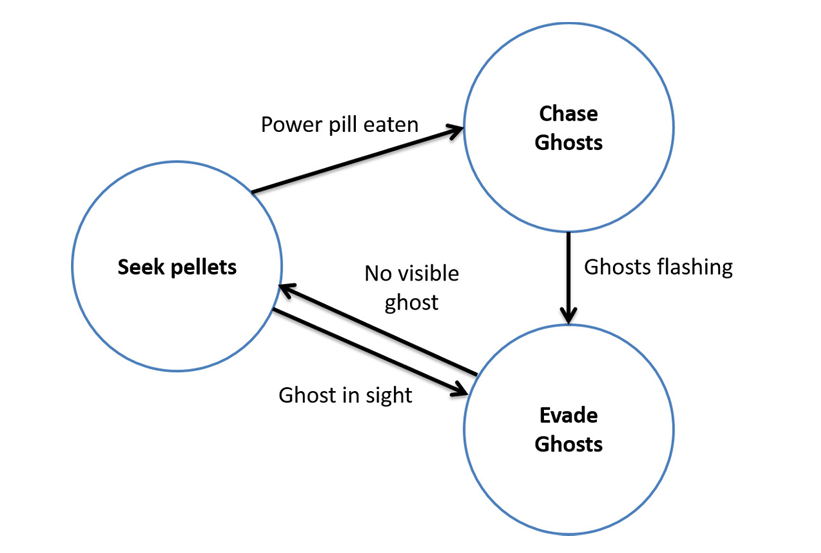
\includegraphics[width = 0.7\textwidth]{Imagenes/FMS_MsPac-man.png}
	\caption{Comportamiento jugador Pac-Man, extraído del libro de Yannakakis y Togelius (2018)}
	\label{fig:Comportamiento jugador Pac-Man}
\end{figure}

Un punto en contra de las FSMs es que son muy inflexibles y estáticas, de manera que las posibilidades de escalado de la lógica son limitadas. También son algo predecibles una vez el jugador ha estudiado los estados y transiciones de una entidad, este punto negativo puede paliarse implementado probabilidades o reglas que no estén tan claras a la hora de hacer las transiciones.

\subsection{Árboles de comportamiento}

Un árbol de comportamiento o Behavior Tree (BT) es un sistema similar a las FSMs ya que contamos con nodos y transiciones y solo uno de esos nodos, que ahora pasan a ser comportamientos en lugar de estados, puede estar activo al mismo tiempo. \\
En esencia, es un árbol de nodos que se organizan jerárquicamente y que atienden a unas normas que controlana el flujo de cambios de nodo. \\

La principal ventaja respecto a las FSMs es su modularidad, la capacidad que tiene un sistema de dividir la lógica del comportamiento en piezas independientes y reutilizables, pudiendo agrupar estas piezas en grupos que a su vez funcionan como una pieza. \\
Su facilidad para ser diseñados y testeados han hecho que los árboles de comportamiento se conviertan en una opción real para modelar IA en la industria del videojuego, con juegos como \textit{Bioshock (2K Games, 2007)}\footnote{\url{https://es.wikipedia.org/wiki/BioShock}} y \textit{Halo 2 (Microsoft Game Studios, 2004)}\footnote{\url{ https://www.gamedeveloper.com/programming/gdc-2005-proceeding-handling-complexity-in-the-i-halo-2-i-ai}} como referencias en el uso de BTs.\\

Un ejemplo no tan conocido de uso de BTs en la industria del videojuego es \textit{Spore (2008, Maxis)}. Spore es un videojuego en el que el jugador va a comenzar creando una célula y va encarnarla durante todo el proceso de su evolución hasta que esta se convierta en un ser mucho más complejo llegando incluso a construir una civilización muy avanzada. La inteligencia artificial de las entidades que nos rodean en este videojuego están fundamentadas en BTs.\\

La gran diferencia de como usa BTs Spore a los juegos anteriormente mencionados es que Spore separa el concepto de \textit{decider} de \textit{behavior}. Los BTs de Halo 2 están compuestos por \textit{behaviors} ya sean estos comportamientos grupales, en los que se elige entre varias opciones, o individuales, que ejecutan acciones específicas, e impulsos que son los saltos que se dan entre comportamientos y que se toman dependiendo de una prioridad, que a futuro resulta en problemas de escalabilidad. Para solucionar este problema, en Maxis deciden unificar el concepto de impulso y comportamientos grupales bajo el nombre de \textit{deciders}, dejando completamente separado el concepto de \textit{behavior} y permitiendo que estos puedan ser reutilizados en múltiples lugares del árbol, asegurando la escalabilidad.\\

La Figura \ref{fig:BT Spore} es un ejemplo de un BT sacado de las documentación\footnote{ \url{https://chrishecker.com/My_Liner_Notes_for_Spore/Spore_Behavior_Tree_Docs}} que hay publicada del juego.
Un punto importante a tener en cuenta es que si un nodo tiene más de un hijo, estos se comprueban si son o no elegidos en un orden determinado hasta que un de los \textit{deciders} acepte la petición del padre o ninguno acepte y se vuelva al nodo actual volviendo a repetir el proceso.\\

\begin{figure}[h]
	\centering
	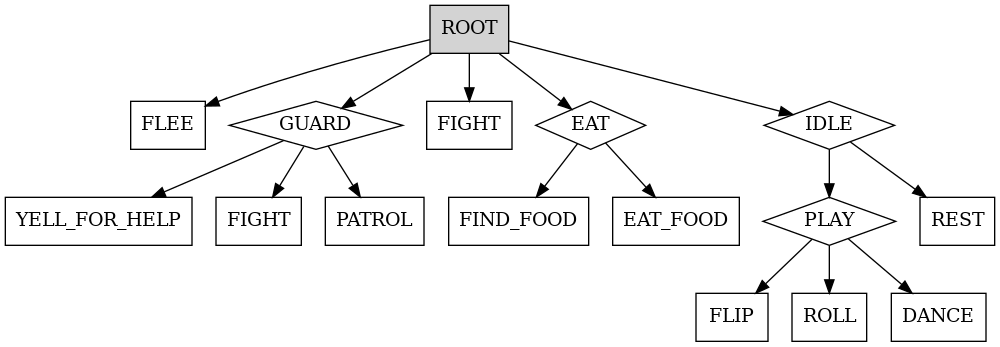
\includegraphics[width = 0.7\textwidth]{Imagenes/BT_Spoore.png}
	\caption{Ejemplo BT, Documentación Spore}
	\label{fig:BT Spore}
\end{figure}
\subsection{Goal-Oriented Action Planning}

GOAP es un sistema basado en planificación de acciones. En lugar de definir comportamientos fijos como hemos visto anteriormente, la entidad analiza la situación y construye un plan óptimo para alcanzar el objetivo designado.
Para que un sistema de esta índole pueda llevarse a cabo deben tenerse una serie de elementos clave.
\begin{itemize}
	 \item Objetivos: lo que la entidad quiera lograr.
	 \item Acciones: conjunto de acciones que la entidad pueda realizar.
	 \item Mundo: estado actual del contexto de la entidad.
	 \item Planificador: encuentra la secuencia óptima de acciones para lograr el objetivo.
\end{itemize}
\comp{https://github.com/crashkonijn/GOAP herramienta que podriamos analizar}\\ 
\subsection{Aprendizaje por Refuerzo (RL) o Redes Neuronales}
\section{Análisis herramientas}
\subsection{Behaviour Bricks}
\subsection{Play Maker}
\subsection{Animator}
\section{Motores de videojuegos}
\subsection{Unity}
\subsection{Unreal}
\subsection{Godot}
\subsection{GameMaker}
\subsection{Construct 3}
\section{Conclusiones}
-----------------------------------------------------\\
En el estado de la cuestión es donde aparecen gran parte de las referencias bibliográficas del trabajo. Una de las formas más cómodas de gestionar la bibliografía en {\LaTeX} es utilizando \textbf{bibtex}. Las entradas bibliográficas deben estar en un fichero con extensión \textit{.bib} (con esta plantilla se proporciona el fichero biblio.bib, donde están las entradas referenciadas más abajo). Cada entrada bibliográfica tiene una clave que permite referenciarla desde cualquier parte del texto con los siguiente comandos:

\begin{itemize}
\item Referencia bibliografica con cite: \cite{ldesc2e}
\item Referencia bibliográfica con citep: \citep{notsoshort}
\item Referencia bibliográfica con citet: \citet{latexAPrimer}
\end{itemize}

Es posible citar más de una fuente, como por ejemplo \citep{latexCompanion,LaTeXLamport,texKnuth}

Después, \LaTeX se ocupa de rellenar la sección de bibliografía con las entradas \textbf{que hayan sido citadas} (es decir, no con todas las entradas que hay en el .bib, sino sólo con aquellas que se hayan citado en alguna parte del texto).

Bibtex es un programa separado de latex, pdflatex o cualquier otra cosa que se use para compilar los .tex, de manera que para que se rellene correctamente la sección de bibliografía es necesario compilar primero el trabajo (a veces es necesario compilarlo dos veces), compilar después con bibtex, y volver a compilar otra vez el trabajo (de nuevo, puede ser necesario compilarlo dos veces). 
